In this section, we describe the overall approach we adopt in this thesis to create a benchmark of executable python software and using this benchmark to generate a data set for training a machine learning model for program analysis and further use this trained model to perform some of the machine learning tasks in program analysis.

The overall workflow of our approach is shown in the Figure \ref{fig:overall_approach}. In the section \ref{approach:selection of projects}, we describe the details on how we select specific projects from the large corpus of python projects. We describe the installation and setup of the selected projects in the section \ref{approach:setup and install}. In section \ref{approach:command line interface} we describe the command line interface and what can be done using it. In section \ref{approach:dynamic analysis} we describe the various dynamic analysis that we can perform to generate data set for program analysis. We describe the machine learning model and its training data in the section \ref{approach:ml model}. Finally, in section \ref{approach:application} we describe how we can use this framework and the trained machine learning model for program analysis.

\begin{figure}[ht]
\centering
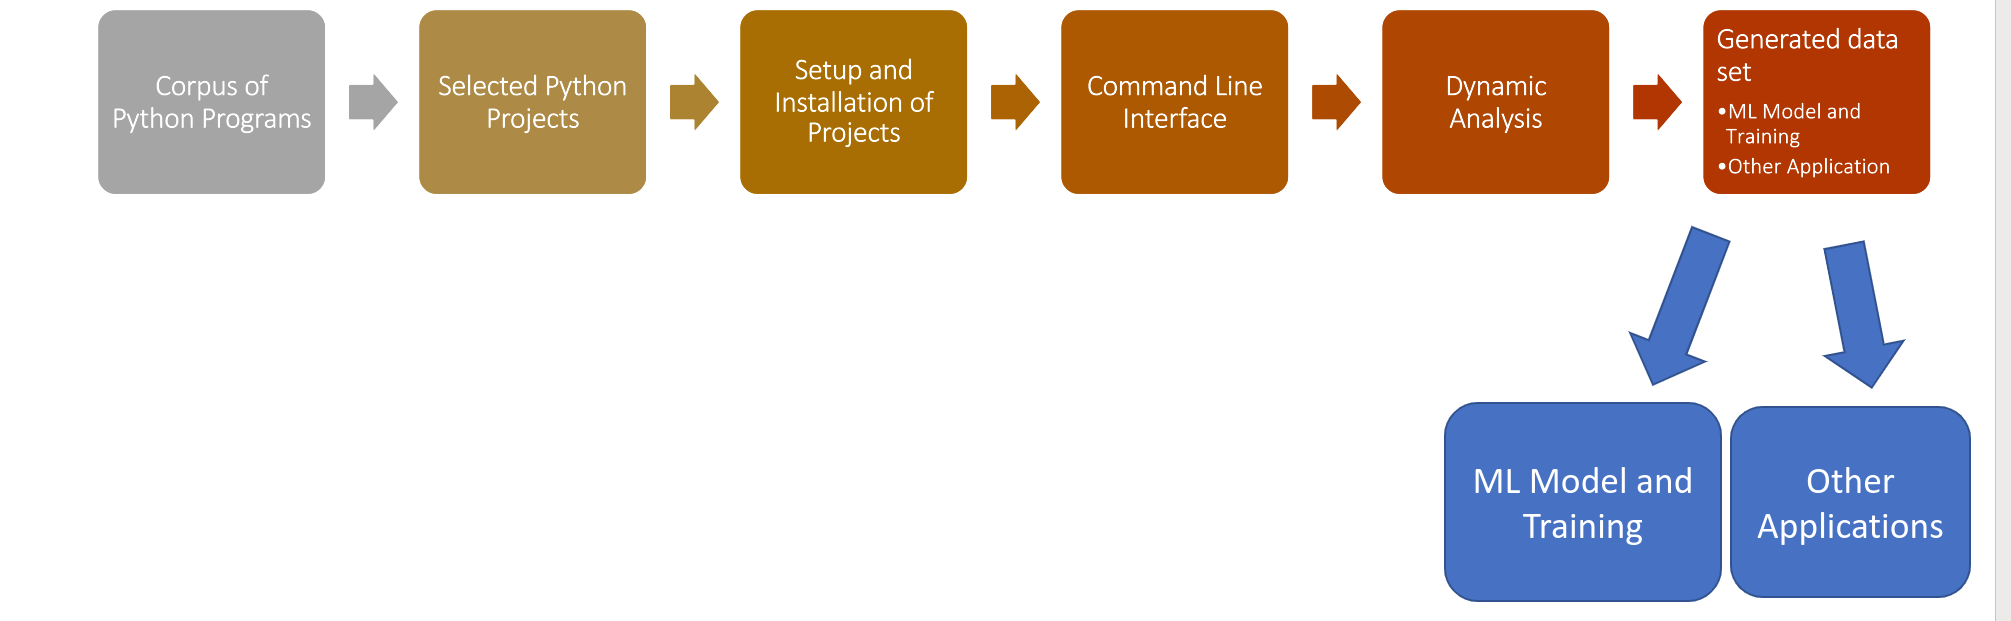
\includegraphics[width=1\linewidth]{figures/approach/Approach2.png}
\caption[Approach]{\label{fig:overall_approach}Overall Approach of DyPyBench.}
\end{figure}

\section{Selected Python Projects}
\label{approach:selection of projects}

\section{Setup and Install}
\label{approach:setup and install}

\section{Command Line Interface}
\label{approach:command line interface}

\section{Dynamic Analysis}
\label{approach:dynamic analysis}

\section{ML Model}
\label{approach:ml model}

\section{Application}
\label{approach:application}